\documentclass{VUMIFInfBakalaurinis}
\usepackage{algorithmicx}
\usepackage{algorithm}
\usepackage{algpseudocode}
\usepackage{amsfonts}
\usepackage{amsmath}
\usepackage{bm}
\usepackage{caption}
\usepackage{color}
\usepackage{float}
\usepackage{graphicx}
% \usepackage{hyperref}  % Nuorodų aktyvavimas
\usepackage{listings}
\usepackage{subfig}
\usepackage{url}
\usepackage{wrapfig}
\usepackage{adjustbox}
%\usepackage{csquotes}
%\usepackage[autostyle,german=guillemets,norwegian=quotes]{csquotes}
\usepackage{dirtytalk}

\usepackage[utf8]{inputenc}
\usepackage[english,lithuanian]{babel}

% Titulinio aprašas
\university{Vilniaus universitetas}
\faculty{Matematikos ir informatikos fakultetas}
\department{Programų sistemų katedra}
\papertype{Baigiamasis bakalauro darbas}
\title{Privačios informacijos išsaugojimas taikant dirbtinio intelekto technologijas}
\titleineng{Privacy-preserving AI}
\status{4 kurso 3 grupės studentas}
\author{Paulius Milmantas}
\supervisor{dr. Linas Petkevičius}
\date{Vilnius \\ \the\year}

% Nustatymai


\begin{document}
\maketitle

\tableofcontents

\sectionnonum{Įvadas}
	%(https://eur-lex.europa.eu/legal-content/LT/TXT/?uri=celex%3A32016R0679)	
	\par Mašininis mokymas yra dirbtinio intelekto sritis, kuri pasitelkia statistinius algoritmus, kad apibrėžtų duomenų generavimo mechanizmą, ar egzistuojančius sąryšius, priklausomybes. Modelis dažnai turi didelį kiekį nežinomų parametrų, kuriuos reikia įvertinti iš duomenų, todėl modelio apmokymui dažniausiai reikia turėti daug duomenų. Kai kurie uždaviniai reikalauja duomenų, kurie nėra laisvai prieinami ir yra privatūs. Mašininio mokymo tyrimų srityje yra kilusi problema dėl jų saugojimo \cite{10}. Vienas iš faktorių, kuris lėmė šį susidomėjimą yra 2016 metais Europos Sąjungoje priimtas duomenų apsaugos reglamentas (GDPR). Pagal jį, fizinių asmenų duomenys turi būti saugomi naudojantis tam tikromis taisyklėmis ir negali būti atskleisti trečiosioms šalims, be asmens sutikimo \cite{1}.
	% https://towardsdatascience.com/perfectly-privacy-preserving-ai-c14698f322f5
	\par Šią problemą išspręsti siekia įvairūs tyrimai ir naujai pasiūlyti metodai privatumą saugančio dirbtinio intelekto srityje. Šią problemą galima išskaidyti į kelias atskiras sritis:
\begin{itemize}
    \item Analizuojamų duomenų privatumas \cite{2}. Algoritmas apmoko modelį atpažinti duomenis. Turint sukurtą modelį, neturi būti galima atgaminti duomenų, pagal kuriuos jis buvo mokomas, bei negali būti identifikuoti asmenys. Taip nukentėtų žmonių privatumas ir būtų pažeistas Europos duomenų apsaugos reglamentas. Šio pažeidimo pavyzdys gali būti ir paprastas teksto atkūrimo modelis. Duodama sakinio pradžia, modelis nuspėja jo pabaigą. Jeigu suvedus tam tikras detales modelis užbaigia sakinį naudodamas asmeninius duomenis, kurie atskleidžia žmonių tapatybę, šis modelis nėra saugus \cite{12}.
    \item Duomenų įvesties privatumas. Trečios šalys neturi matyti įvedamų duomenų. Tai gali būti tinklo saugumo spragos, duomenų surinkimo aplikacijų spragos ir t.t…
    \item Modelio išvesties privatumas. Modelio išvesties neturi matyti asmenys, kuriems šie duomenys nepriklauso. Šis punktas yra sąlyginis, priklauso nuo modelio svarbos. Jeigu tai yra svarbūs asmeniniai duomenys, negalima rizikuoti. Tačiau jeigu tai yra viešai prieinami duomenys, šis punktas negalioja.
    \item Modelio apsauga. Sukurtas modelis negali būti niekieno pasisavintas. Šis punktas yra skirtas apsaugoti programos kūrėją.
\end{itemize}

	% https://www.nature.com/articles/s42256-020-0186-1 [Nepanaudotas]
	% https://towardsdatascience.com/the-new-dawn-of-ai-federated-learning-8ccd9ed7fc3a
	\par Darbo tikslas - ištirti ir palyginti privatumą saugančius dirbtinio intelekto algoritmus pagal jų saugumą, našumą ir panaudojamumą, bei pateikti rekomendacijas.
	\par Darbo uždaviniai:
	\begin{itemize}
		\item Išanalizuoti esamus algoritmus pagal jų saugumą ir panaudojamumą.
		\item Ištirti kurie algoritmai yra realizuoti realizuoti algoritmus, kurie nėra atvirai prieinami.
		\item Palyginti algoritmus pagal našumą.
	\end{itemize}
\section{Asmens duomenų privatumas mašininio mokymo kontekste}
	\par Vienas iš būdų apsaugoti duomenis yra decentralizuoti modelį ir naudoti paskirstyto mokymo algoritmus. Paprastai mašininiam mokymui yra naudojamas centralizuotas serveris. Yra surenkami duomenys į vieną vietą ir modelį moko vienas kompiuteris. Jeigu norima pridėti daugiau duomenų arba papildomą klasifikatorių, modelį reikia apmokyti iš naujo. Taip pat, kas kuria šį modelį, turi visą prieigą prie duomenų, šie modeliai nėra saugūs \cite{13}. 
	\par Šiai bėdai išspręsti, vienas iš metodų yra federuotas mašininis mokymas (\say{Federated machine learning}). Šis metodas padeda išspręsti kaikurias bėdas, vykdant modelio mokymą decentralizuotai \cite{3}. Prie bendro tinklo gali prisijungti daug įrenginių. Visi jie turi savo unikalų duomenų rinkinį. Kiekvienas įrenginys pasirenka geriausią statistinį metodą modelio mokymui ir pagal tą metodą sukuria modelį. Taip yra sukuriama daug skirtingų modelių, realizuotų su skirtingais duomenų rinkiniais. Visi šie rinkiniai vėliau yra surenkami į vieną vietą ir toliau naudojami duomenų analizei. Taip surinkus atskirų įrenginių sukurtus modelius, neturime prieigos prie pradinių duomenų ir daugiau žmonių gali prisidėti prie modelio kūrimo, nematant pilno duomenų rinkinio. Tačiau naudojant šį metodą ne visos problemos yra išsprendžiamos. Duomenų saugumas nėra garantuojamas \cite{3}. Jeigu duomenys nėra užšifruojami, jie gali būti pavogti. Tai gali būti padaryta, jeigu yra naudojamas nesaugus interneto ryšys, arba jeigu yra bandoma analizuoti atskirų įrenginių atsiųstus modelius. Šis metodas išsprendžia tik kelias problemas. Likusios yra: komunikavimo kaštai, įrenginių heterogeniškumas, statistinis heterogeniškumas ir saugumo problemos \cite{4}.
%https://www.researchgate.net/publication/335319008_Federated_Learning_Challenges_Methods_and_Future_Directions [Nepanaudotas]
	\par Visos šios problemos yra nagrinėjamos ir joms spręsti kuriami nauji metodai. Komunikacijos kaštams mažinti, yra kuriami algoritmai, kaip turi būti perduodamas modelis tinkle, kad būtų maža tinklo apkrova. Įrenginių heterogeniškumui spręsti, yra parenkami tam tikri įrenginių rodikliai ir pagal tai nustatoma, kokia bus įrenginio komunikacija: ar jis naudos asinchroninį komunikavimą, kaip dažnai tai vyks ir kokia yra įrenginio klaidos tikimybė \cite{4}. Statistikos heterogeniškumui pataisyti kuriami yra metodai, kaip meta duomenų-mokymas ir keletos užduočių mokymas (\say{Multi-task learning}). 
	% https://arxiv.org/pdf/1906.10893.pdfmif
	\par Straipsnyje apie privatumą išsaugančius blokų-grandinių tinklus (\say{Privacy-Preserving Blockchain-Based Federated Learning for IoT Devices}) yra pateikiamas naujas paskirstyto mokymosi algoritmas, kuris yra paremtas
blokų grandinių technologijomis \cite{5}. Šis modelis yra grafiškai pateiktas pav.1. Šią architektūrą pavyzdyje sudaro 3 komponentai: gamintojai, klientai ir blokų gradinių tinklas. Šiame pavyzdyje gamintojas pareiškia užklausą, kad reikia atlikti apklausą. Klientai, kurie sutinka su užklausa, išsiunčia savo sukurtą modelį. Blokų grandinių tinklas elgiasi kaip centralizuotas serveris ir surenka visus klientų modelius. Tuomet, pasirinktas kompiuteris, kuris atlieka visą darbą (\say{miner}) atlieka galutinį modelių sujungimą.


\begin{figure}[ht]
  \centering
  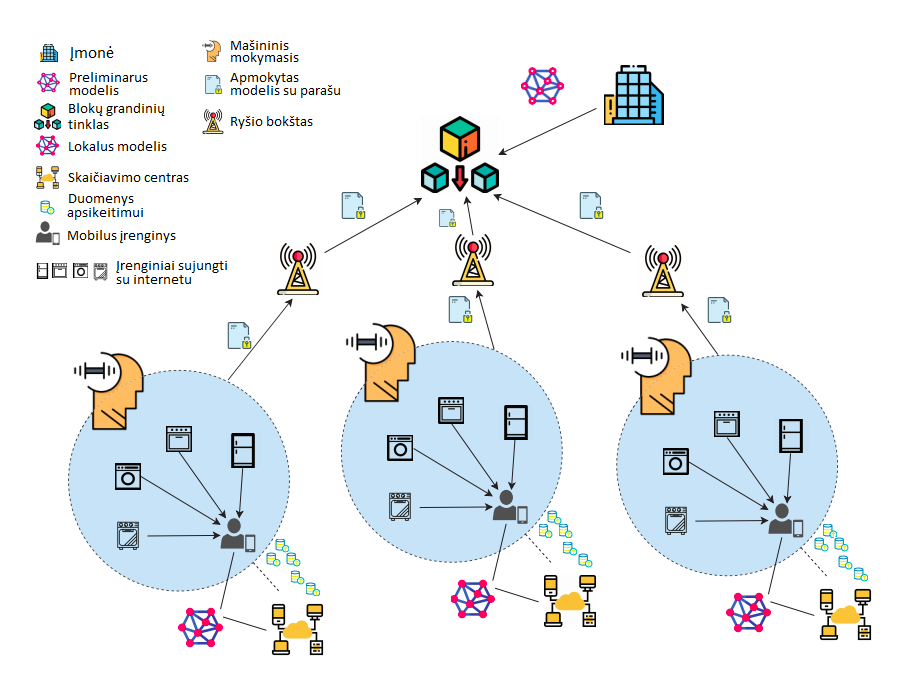
\includegraphics[width=13cm,height=11cm,keepaspectratio]{img/paskirstytasMokymasis.png}
  \caption{Paskirstytas mokymas \cite{5}}
  \label{fig:overflowProblem}
\end{figure}

% https://www.inpher.io/technology/what-is-secure-multiparty-computation
\par Minėti decentralizuoti būdai apjungia skirtingus sukurtus modelius į vieną ir visi įrenginiai kurie kuria modelius, naudoja savo unikalius duomenis. Saugus skirtingų pusių skaičiavimo metodas (\say{Secure multiparty computation}) yra kriptografinis protokolas, kuris leidžia įrenginiams, su unikaliais duomenimis, skaičiuoti funkcijos reikšmę, nematant kitų įrenginių reikšmių \cite{6}. Su šiuo metodu, yra sukuriamas vienas modelis tarp įvairių įrenginių. Pagrindinis įrenginys, kuris ruošia skaičiavimo užklausą, gali suskaidyti pradinius duomenis, užšifruoti juos ir taip paskirstyti tarp kitų įrenginių. Taip sukurti įrenginio rezultatai negali būti atšifruoti ir pasisavinti, o minėto federuoto mokymo metodo sukurti rezultatai, jeigu nėra gerai apsaugoti, gali būti pasisavinti ir atgauti pradiniai duomenys su kuriais modelis buvo sukurtas.
% https://www.researchgate.net/publication/236935821_Homomorphic_Encryption_Theory_Applications
\par  Kitas būdas apsaugoti modelį yra naudoti homomorfinį šifravimą. Pagal šį metodas, modelis yra mokomas naudojant užšifruotais duomenimis. Jie mokymo metu, nėra atšifruojami. Šis metodas leidžia keliems įrenginiams vienu metu atlikti skaičiavimus su duomenimis, kurių jie nemato. Yra daug metodo varijacijų. Kaikurios yra pažeidžiamos ir gali atskleisti visos infrastruktūros duomenis \cite{7}. Dažniausiai homomorfinės sistemos yra labiau pažeidžiamos nei nehomomorfinės.
% https://eprint.iacr.org/2016/421.pdf
\par 2016 metais buvo pasiūlytas naujas metodas paspartinti pilnai homomorfines šifravimo sistemas \cite{8}. Homomorfinės sistemos, kurios naudoja šį metodą yra laikomos ketvirtos kartos. Šis metodas leidžia aproksimuoti užšifruoto teksto sudėtį, daugybą ir pakeisti atšifruoto teksto proporcijas. 
Proporcijų pakeitimo procedūra suskaido užšifruotą tekstą į dalis, to pasekoje yra apvalinamas neužšifruotas teksas. Šio metodo pagrindinė idėja yra pridėti triukšmo prie pagrindinės žinutės. Šis triukšmas yra pridedamas prie neužšifruoto teksto dėl saugumo priežasčių ir jis yra laikomas kaip aproksimavimo paklaida. Tuo pasekoje, metodas veikia su tam tikra paklaida
% https://www.inpher.io/technology/what-is-secure-multiparty-computation
\par Bendro įspūdžio agregavimo metodas yra naujausias iš visų minėtų. Jis leidžia įrenginiui su savo duomenimis sukurti modelį naudojant betkokius metodus ir taip prisidėti prie bendro progreso \cite{6}. Visi modeliai yra surenkami ir leidžiami duomenys per šiuos modelius. Kiekvienas modelis skiria savo balsą, jie surenkami ir padaromas bendras sprendimas. Šis metodas leidžia lengvai plėsti modelį. Taip pat yra saugomas ir duomenų privatumas. Jeigu keli modeliai, kurie nesidalina duomenimis, teigia vienodai, tai reiškia, kad negalima atkurti duomenų ir jie yra saugūs. Skaičiavimas vykdomas pasirenkant optimalią strategiją ir imant mažiausią galimą žingsnių skaičių.

%https://www.researchgate.net/publication/335319008_Federated_Learning_Challenges_Methods_and_Future_Directions – kylančios problemos

%https://www.researchgate.net/publication/236935821_Homomorphic_Encryption_Theory_Applications

%Idomus straipsnis apie block chain technologijas
%https://arxiv.org/pdf/1906.10893.pdf

%Apie galimybe nulauzti modeli
%https://arxiv.org/abs/1911.07135

\section{Duomenų pažeidžiamumo metrikos}

\subsection{Apibrėžimas}
\par Norint apsaugoti duomenis, sukurtam duomenų aptikimo modeliui reikia atlikti analizę, kaip tikėtina, kad modelio pradiniai duomenys bus atkurti. Tai išanalizuoti yra daug būdų, vienas iš jų yra pateiktas straipsnyje \cite{11}.
 Šis straipsnis ieško metrikos reikšmės, kuri parodo, kaip pradinius duomenis atsimena modelis.
\par Tarkime turime duomenų rinkinį s[r]. Šiam rinkiniui pirma reikia apskaičiuoti rangą.

\begin{equation}
rangas(s[r]) = | {r` \in R : Px(s[r`]) \leq Px(s[r])} |
\label{eq:Lygtis 1.}
\end{equation}
Čia funkcija $Px$ -- logaritminis entropijos matas, kuris nusako, ar modeliui paduoti duomenys yra tipiniai, ir ar modelis buvo matęs panašius duomenis. Didesnė $Px$ reikšmė reiškia, kad modelis panašių duomenų nebuvo matęs, o mažesnė reikšmė reiškia, kad panašius duomenis modelis yra matęs. Logiritminės entropijos formulė pateikta lygtyje [2]. $s[.]$ -- yra pradinis duomenų rinkinys. Skaičius skliaustuose parodo, kuriuos duomenis reikia paimti iš rinkinio.

\begin{equation}
Px_{\theta}(x_{1}, ..., x_{n}) = -\log_{2} Pr(x_{1}, ..., x_{i - 1} | f_{\theta})
\label{eq:Lygtis 2.}
\end{equation}
Čia formulė $Pr$ -- nežinomas skirstinys. Jeigu skaičiuotume funkciją $Pr(x_{i} | x_{1}, ..., x_{n})$, gautume tikimybę, kad $x_{i}$ atsiranda po reikšmių, nuo $x_{1}$ iki $x_{i-1}$

\par Šis rangas nurodo, kurioje vietoje yra šis inicijuotas duomenų rinkinys sąraše, tarp visų galimų testinių rinkinių kombinacijų. Pavyzdžiui, norima 
sukurti natūralios kalbos atpažinimo modelį. Jo mokymui, yra paduodamas atsitiktinai sugeneruotas sakinys \say{Atsitiktinis skaičius 125} ir apskaičiuojama jo entropija. Tada galima išrašyti visus galimus sakinius, kuriuos yra leidžiama siųsti, ir juos surūšiuoti pagal entropijos laipsnį. Tada reikia apskaičiuoti, kaip dažnai pasitaiko panašūs sakiniai. Taip yra gaunamas rangas. Kadangi šis pavyzdinis sakinys yra sudėtingas, su atsitiktiniais skaičiais ir jo entropija yra aukšta, tikriausiai aukštesnė nei dauguma mokymo duomenų, jo rangas bus artimas vienetui. Darant prielaidą, kad šio sakinio entropija yra pati aukščiausia iš galimų testavimo duomenų, galima teigti, jog šio sakinio rangas yra lygus vienetui.
\par Rangas tiesiogiai nepasako kokia yra tikimybė, kad bus sugeneruotas toks testavimo rinkinys. Jo skaičiavimas paima daug resursų, nes reikia sugeneruoti visas galimas kombinacijas \cite{11}.
\par Kitas nagrinėjamas kintamasis yra \say{atvirumo} metrika. Tai aproksimacija, kuri nusako, kaip tikėtina, jog testavimo duomenys bus atgaminti iš modelio. Ši metrika pasako ką naujo sužinome apie pradinius duomenis, kai per modelį paleidžiame atsitiktinai sugeneruotus duomenis. Todėl, reikia skaičiuoti prognozuojamą entropiją, pagal pateiktas modelio prognozes. Prognozės entropija, tai spėjimų skaičius $E(X)$, kuris reikalingas atspėti diskretų, atsitiktinai sugalvotą parametrą X.
% https://www.usenix.org/system/files/sec19-carlini.pdf % 
\par Jeigu kintamasis r yra pasirenkamas atsitiktinai $r \in R$, tai reiškia, kad reikia generuoti atsitiktinius skaičius tol, kol bus gauta r reikšmė. Iš to seka, kad spėjimų turėtų būti lygus [3] lygčiai.

\begin{equation}
E(s[r])_{\theta} = \frac{1}{2} | R |
\label{eq:lygtis3}
\end{equation}

\par Turint suskaičiuotus galimus rinkinių rangus, bei entropijas, galima naudoti patobulinta skaičiavimo taktiką. Visi galimi duomenys yra surušiuojami pagal entropiją arba sudėtingumą. Sąrašo pradžioje yra elementas su mažiausia entropija. Jo atspėjimo tikimybė yra viena iš didžiausių. To pasekoje, gauname formulę [4].

\begin{equation}
E(s[r]|f_{\theta}) = rank_{\theta}(s[r])
\end{equation} 

\par Ši formulė padidina skaičiavimų spartumą ir tai galima apskaičiuoti padalinus vieną formulę iš kitos. Tai pateiktas [5] lygtyje.

\begin{equation}
\frac{E(s[r])}{E[s[r]|f_{\theta}]} = \frac{\frac{1}{2}|R|}{rank_{\theta}(s[r])}
\end{equation}

\par Rangai tiksliai neapibrėžia kokia yra tikimybė, jog elementas bus atspėtas. Jis tik lygina visas galimas kombinacijas ir skaičiuoja jų entropijas. To pasekoje, visi šie skaičiavimai yra tik apytikslis spėjimas. Kadangi tai nėra tikslu ir norima sužinoti tik bendrą vaizdą apie algoritmą, galima naudoti logaritmus. Tai atlikta lygtyje [6].

\begin{equation}
log_{2}(\frac{E(s[r])}{E(s[r]|f_{\theta})}) = log_{2}(\frac{\frac{1}{2}|R|}{rank_{\theta}(s[r])})
\end{equation}

\par Šias lygtis supaprastinus, gaunama lygtis [7].

\begin{equation}
log_{2}|R| - log_{2}(rank_{\theta}(s[r])) - 1
\end{equation}

\par Dėl paprastumo yra pridedamas vienetas ir taip gaunama atvirumo metrika, pateikta lygtyje [8].

\begin{equation}
atvirumas(s[r])_{\theta} = \log_2 | R | - \log_2 rangas_{\theta}(s[r])
\end{equation}
\subsection{Skaičiavimas praktikoje}
\par Pažeidžiamumo metrika \say{Atvirumas} yra naudojama tikrinant mašininio mokymo algoritmų duomenų įsiminimą. Atlikus šiuos skaičiavimus, programuotojai gali spręsti dėl tolimesnių veiksmų: tęsti kūrimą ar dirbti ties duomenų anonimizavimu.
\par Mašininio mokymo algoritmo tikrinimui su atvirumo metrika, pirma reikia pasiruošti duomenų rinkinį s[r]. Sudarius šį rinkinį, reikia sukurti mašininio mokymo modelį. Turint gautą modelį ir duomenis, kurie buvo naudojami modelio gavimui, galima skaičiuoti atvirumo metriką. Siekiant daugiau sužinoti apie modelį, galima savo duomenis įterpti daugiau nei vieną kartą. Pavyzdžiui, jeigu vienus duomenis įterpsime kelis kartus, o kitus duomenis šimtą kartų, galima analizuoti atvirumo metriką su šiais duomenimis. Taip galima gauti abstrakčią koreliaciją tarp duomenų kiekio ir modelio atsiminimo. Kad šie eksperimentai būtų tikslūs, būtina kiekvieno modelio kūrimo metu naudoti tuos pačius parametrus: optimizavimo funkcijas, hiperparametrus ir kitus duomenis. Taip su kiekvienu pavyzdiniu duomenų rinkiniu, turi būti atlikta atskira analizė. Jeigu galima, turi būti didinamas vienodų duomenų kiekis ir tikrinama atvirumo ir žinomų duomenų kiekio koreliacija.
\par Atvirumui sužinoti, reikia skaičiuoti rangą. Tikslaus jo radimo procedūros nėra. Todėl reikia naudotis analitiniais metodais. Vienas iš jų yra aproksimacija pagal distribucijos modelius. Tarkime, turime duomenis, kurių entropija yra didesnė, nei s[r] duomenų. Reikia rasti kiek yra tokių duomenų, kurių entropija yra mažesnė. Taip pat, tarkime, kad s[r] entropija yra $\rho(.)$ pasiskirstymo distribucijos. Atvirumą galima aproksimuoti skaičiuojant šio skirstinio plotą grafike, iki testavimo duomenų, ir dauginant iš logaritmo.
Taip gauname formulę [9].

\begin{equation}
atvirumas(s[r])_{\theta} = -log_{2} \int_{0}^{Px_{\theta}(s[r])} \rho(x)dx
\end{equation}

\subsection{Iliustacinis pavyzdys}
\par Metodo panaudojamumą pademonstruoti, pasinaudokime mašininiu modeliu, pagrįstu cukriniu diabetu sergančių moterų duomenimis. Modelis priima 5 parametrus: nėštumų skaičių, gliukozės kiekį kraujyje, kraujo spaudimą, BMI ir amžių. Visų šių parametrų ribos yra žinomos, todėl turint atsitiktinių duomenų rinkinį, galima apskaičiuoti rangus. Todėl bus naudojama lygtis [10], turinti rangus.

\begin{equation}
atvirumas(s[r])_{\theta} = \log_{2}|R| - \log_{2}rangas_{\theta}(s[r]) 
\end{equation}

\par Tarkime, kad šių duomenų galimos ribos yra tokios: nėstumai: [0-30], gliukozės kiekis kraujyje: [0-180], kraujo spaudimas: [0-250], BMI: [1-70], amžius: [1-110]. Suskaičiuoti kiek iš viso yra galimų variantų, galima sudauginus visas šias ribas, tai padaryta lygtyje [11].

\begin{equation}
R = 30 \cdot 180 \cdot 250 \cdot 69 \cdot 109 = 10153350000
\end{equation}

\par Tarkime, turime dviejų žmonių testinių duomenų rinkinį. Pirmo žmogaus duomenys: [2, 60, 98, 25, 25], antro: [0, 90, 128, 27, 18]. Skaičiuojame rangus [12] ir [13]. Vėliau pagal apskaičiuotus rangus, ieškoma atvirumo metrika [14] ir [15].

\begin{equation}
s[1] = 2*180*250*69*109 + 60*250*69*109 + 98*69*109 + 25*109 + 25 = 790444808
\end{equation}
\begin{equation}
s[2] = 90*250*69*109 + 128*69*109 + 27*109 + 18 = 170188149
\end{equation}
\begin{equation}
atvirumas(s[1]) = log_{2} 10153350000 - log_{2} 790444808 = 3.68314726
\end{equation}
\begin{equation}
atvirumas(s[2]) = log_{2} 10153350000 - log_{2} 170188149 = 5.89868142
\end{equation}

\par Pagal rezultatatus, galima teigti, kad yra labiau tikėtina, kad bus atskleisti antro žmogaus duomenys. Turint daugiau parametrų, būtų dar mažesnė atvirumo metrikos reikšmė, nes būtų dar mažiau tikėtina, kad bus atkartoti duomenys. Turint kelius modelius, galima lyginti modelių atvirumo metrikas ir spręsti apie modelių saugumą.

\section{Modelių palyginimo metodai}

\subsection{Lyginimas pagal duomenų nuokrypį}

\par Siekiant palyginti, kaip modeliai gerai saugo privačius duomenis, apibrėžiame metriką DMDK (didžiausias modelio duomenų nuokrypis). Kuo metrika yra mažesnė, tuo tiksliau galima nuspėti, kokie duomenys buvo naudojami modelio mokymui. Kuo metrika didesnė, tuo yra sunkiau nuspėti, kokie duomenys buvo naudojami mokymui. Ši metrika leidžia lyginti skirtingus modelius su skirtingais duomenimis. Metrika buvo sugalvota specialiai šiam darbui, siekiant palyginti skirtingus modelius.
\par DMDK yra išvestas lygtyje [16]. Prieš DMDK skaičiavimą reikia paimti visus modelio mokymui skirtus duomenis ir kiekvienai duomenų eilutei apskaičiuoti modelio išvestį. Skaičiavimus reikia atlikti tik su tomis eilutėmis, su kuriuomis modelis išvedė teisingą atsakymą. Turint tik tas eilutes, su kuriomis modelis išvedė teisingą atsakymą, galima į nelygybę įstatyti kintamuosius. Lygtyje yra naudojami tokie kintamieji: m - duomenų eilučių skaičius, h - parametrų skaičius (stulpeliai), $\epsilon$ - ieškomas didžiausias galimas kintamasis, su kuriuo modelis nepakeičia išvesties rezultatų, $D_{eilut.:n, stulp.:k}$ - duomenys n eilutėje ir k stulpelyje.

\begin{equation}
DMDK = {\sum_{n=0}^{m} ({\sum_{k=0}^{h} (max((|\epsilon| + D_{eilut.:n, stulp.:k}) : \epsilon \in R))}/{h})}/{m}
\end{equation} 

\subsection{Skaičiavimo pavyzdys}
\par Tarkime egzistuoja modelis, kuris turi 2 parametrus: gliukozės kiekis kraujyje ir KMI. Pagal šiuos du parametrus modelis išveda rezultatą: ar žmogus serga cukriniu diabetu ar ne. Paimamos visos mokymo duomenų eilutės, su kuriomis modelis išveda teisingą rezultatą. Tarkime, jos yra aprašytos \ref{tab:my-table} lentelėje.

\begin{table}[h]
\centering
\begin{tabular}{|l|l|l|}
\cline{1-3}
Gliukozė & KMI  & Išvestis \\\cline{1-3}
148      & 33.6 & 1        \\\cline{1-3}
85       & 26.6 & 0        \\\cline{1-3}
183      & 23.3 & 1        \\\cline{1-3}
\end{tabular}
\caption{Pavyzdiniai duomenys}
\label{tab:my-table}
\end{table}

\par Taikant jau sukurtą modelį, įvertiname ar keičiasi išvestis didinant kiekvienos eilutės kiekvieno stulpelio reikšmes, pridedant $\epsilon$. Kiekvienai reikšmei yra atskirai didinamas $\epsilon$, kol gaunamas tos eilutės tam tikro stulpelio maksimalus $\epsilon$. Skaičiavimams parodyti, tarkime, kad gautos maksimalios $\epsilon$ reikšmės yra pateiktos lentelėje [2].

\begin{table}[t]
\centering
\begin{tabular}{|l|l|l|}
\cline{1-2}
Gliukozė & KMI \\\cline{1-2}
3      & 2 \\\cline{1-2}
6       & 1 \\\cline{1-2}
4      & 0.1 \\\cline{1-2}
\end{tabular}
\caption{Pavyzdinės epsilon reikšmės}
\label{tab:my-table}
\end{table}

\par DMDK skaičiavimas pateiktas lygtyje [17].

\begin{equation}
DMDK = \frac{3 + 2}{2} + \frac{6 + 1}{2} + \frac{4 + 0.1}{2} = 8.05
\end{equation}

\par Apskaičiavus kitų modelių DMDK reikšmes, galima lyginti, kuris modelis efektyviau saugo duomenis, naudotus mokymosi metu. Jeigu kito modelio apskaičiuota DMDK reikšmė būtų didesnė už 8.05, reikštų, kad tas modelis labiau saugo duomenų privatumą.

\subsection{Algoritmo verifikavimas}
\par Siekiant įrodyti, kad algoritmas teisingai įvertina skirtingus modelius ir galima juos palyginti tarpusavyje, paimkime kelis skirtingus modelių pavyzdžius.
\par Tarkime, kad pirmas modelis turi viena parametrą - KMI. Pagal šį parametrą, modelis prognozuoja, ar žmogus serga cukriniu diabetu ar ne. Modelio tikslumas yra 54\%, jis visą laiką prognozuoja, kad žmogus serga cukriniu diabetu. Skaičiuojant DMDK, reikia pasirinkti tik tuos duomenis, su kuriais buvo išvesta teisinga prognozė. Modelis visą laiką prognozuoja, kad žmogus serga cukriniu diabetu, todėl, nėra tokios reikšmės, kurią pridėjus prie duomenų, pasikeis modelio prognozė. Todėl DMDK reikšmė yra $\infty$ ir tai reiškia, kad modelis negali būti saugesnis. Kai modelio prognozė visą laiką yra tapati, neįmano atgaminti pradinių duomenų, su kuriais modelis buvo mokomas.
\par Antras pavyzdinis modelis prognozuoja ar žmogus serga cukriniu diabetu, pagal 2 parametrus: KMI ir gimdymų skaičiumi. Modelio tikslumas yra 72\%, modelio DMDK reikšmė yra 0,00134. Sprendžiant pagal DMDK, modelis yra nesaugus ir yra labai priklausomas nuo pradinių duomenų, su kuriais modelis buvo mokomas. Modelio nesaugumui įrodyti, paimkime kelias savo sugalvotas duomenų eilutes ir pabandykime atgaminti pradinius duomenis. Tarkime, kad mūsų sugalvotos duomenų eilutės yra lentelėje [3].

\begin{table}[h]
\centering
\begin{tabular}{|l|l|l|}
\cline{1-2}
KMI & Gimdymų skaičius \\\cline{1-2}
25      & 3 \\\cline{1-2}
23       & 2 \\\cline{1-2}
\end{tabular}
\caption{Sugalvotos duomenys reikšmės modelio tikrinimui}
\label{tab:my-table}
\end{table}

\par Kiekvienai sugalvotai duomenų eilutei, analizuojame kiekvieną stulpelį. Prie stulpelio reikšmės pridedame $\epsilon$ ir didiname $\epsilon$ reikšmę tol, kol pasikeičia modelio rezultatas. Analizuojame kiekvieną stulpelį ir pasirenkame stulpelį su mažiausia $\epsilon$ reikšme. Pakeičiame analizuojamos duomenų eilutės stulpelio reikšmę, su kuria gauname mažiausią $\epsilon$ reikšmę. Išanalizuokime pirmą duomenų eilutę lentelėje [3]. Po pirmos iteracijos, gauname pakeistą duomenų eilutę: KMI - 26, gimdymų skaičius - 3. Atliekame iteracijas tol, kol gaunamų naujų reikšmių skirtumas tampa labai mažas. Atlikus visų duomenų analizę, gauname duomenis, kurie buvo gauti iš sugalvotų duomenų eilučių. Jeigu modelio DMDK yra mažas, šie duomenys turi būti artimi pradiniams duomenims, kurie buvo naudojami modelio mokymui. Atlikus analizę buvo gauti duomenys lentelėje [4]. Duomenys yra labai panašūs pradiniams modelio duomenims. Tai reiškia, kad DMDK matavimo algoritmas pasiteisino.

\begin{table}[h]
\centering
\begin{tabular}{|l|l|l|}
\cline{1-2}
KMI & Gimdymų skaičius \\\cline{1-2}
26      & 1 \\\cline{1-2}
22       & 2 \\\cline{1-2}
\end{tabular}
\caption{Sugalvotos duomenys reikšmės modelio tikrinimui}
\label{tab:my-table}
\end{table}

\par Siekiant įsitikinti, kad algoritmas yra teisingas ir neduoda rezultatų, kurie tiesiogiai priklauso nuo duomenų, atlikti du eksperimentai.

\begin{enumerate}
    \item Skaitant duomenis, jų visų reikšmės yra padalintos iš 10. Sukūrus modelį, apskaičiuota nauja DMDK reikšmė. Ji yra labai artima DMDK reikšmei, kai duomenys nebuvo dalijami iš 10. Tai reiškia, kad algoritmas nėra tiesiogiai priklausomas nuo duomenų, kuriais modelis yra mokomas.
    \item Skaitant duomenis, prie jų reikšmių yra pridedamas atsitiktinai sugeneruotas triukšmas - skaičius nuo -1 iki 1. Naudo modelio DMDK reikšmė yra panaši į modelio, prieš duomenų keitimą. Tendencijos išlieka panašios.
\end{enumerate}














\section{Homomorfinis šifravimas}
% https://www.venafi.com/blog/homomorphic-encryption-what-it-and-how-it-used %
\par Homomorfinis šifravimas, yra šifravimo algoritmų klasė, kuri yra grindžiama principu, leidžiančiu atlikti skaičiavimus su užšifruotais duomenimis, jų neatšifruojant. Šie algoritmai yra šiek tiek panašūs į viešo šifravimo algoritmus, kurie yra paplitę tinklalapių apsaugoje. Yra naudojamas viešas ir privatus raktas. Su viešu raktu duomenys yra užšifruojami, o su privačiu, atšifruojami. Momomorfinis šifravimas skiriasi nuo viešo šifravimo tuo, kad naudoja algebrainę sistemą, kuri leidžia atlikti skaičiavimus su užšifruotais duomenimis.
  % https://planetmath.org/algebraicsystem %
\par Algebrainė sistema yra duomenų rinkinys kartu su savo matematinėmis operacijomis. 



\par Yra trijų tipų homomorfiniai šifrai: dalinai homomorfiniai (PHE), šiek tiek homomorfiniai (SHE) ir pilnai homomorfiniai šifrai (FHE). Dalinai homomorfinės sistemos leidžia atlikti skaičiavimus visiems duomenims, tik su pasirinkta operacija. Tai gali būti arba sudėtis arba daugyba.  Operacijos duomenims gali būti atliktos neribotą kartą.  Šiek tiek homomorfinės sistemos (SHE) naudoja vieną operaciją iki tam tikro sudėtingumo. Šios operacijos gali būti atlikto ribotą kartų skaičių. Pilnai homomorfinės sistemos leidžia naudoti sudėtį ir daugybą vienu metu, neribotą kartų. 
% https://cryptosith.org/michael/data/talks/2012-01-10-MSR-Cambridge.pdf %
\par Homomorfinių sistemų saugumas yra paremtas žiedinio mokymo su klaidomis problema (\say{Ring learning with errors}).













\section{Federuotas mašininis mokymas}
\subsection{Metodas}
\subsection{Komunikacijos kaštų mažinimas}
\subsection{Įrenginių heterogeniškumas}
\subsection{Analizės heterogeniškumas}
\subsection{Saugos problemos}

\section{Blokų-grandinių technologija}

\section{Saugus skirtingų pusių skaičiavimas}

\section{Bendro įspūdžio privatus agregavimas}

\section{Tyrimas}
\subsection{Modelių palyginimas}

\par Tyrimo tikslams, buvo sukurti modeliai ir, skaičiuojant DMDK metriką, jie lyginami tarpusavyje. Gauti rezultatai pateikti lentelėje [5].

\begin{table}[h]
\begin{adjustbox}{width=\textwidth,center=\textwidth}
\begin{tabular}{|l|l|l|l|}
\cline{1-4}
Modelis & Nuostolių f-jos reikšmė (MSE) & Tikslumas & DMDK  \\\cline{1-4}
PyTorch neuroninis tinklas & 103.9837813 & 81.1\% & 87.419  \\\cline{1-4}
Gradientinio nuolydžio algoritmas & 2272.06 & 63.78\% & 0.051792 \\\cline{1-4}
Pallier homomorfiniu šifravimu grįstas modelis & 2185.37 & 63.52\% & 0.1416 \\\cline{1-4}
\end{tabular}
\end{adjustbox}
\caption{Sugalvotos duomenys reikšmės modelio tikrinimui}
\label{tab:my-table}
\end{table}

\par Pagal gautus rezultatus, pateiktus lentelėje [5], gautos išvados:
\begin{itemize}
    \item PyTorch neuroninis tinklas greičiau artėja prie nuostolių funkcijos minimumo, nei kiti modeliai. Esant ~70\% modelių tikslumui, PyTorch modelis yra saugiausias. Mažiausiai saugus yra paprastu gradientiniu nuolydžiu grįstas modelis. 
    \item Palliers kriptografija grįstas modelis yra saugesnis už paprastą gradientinio nuolydžio metodą.
    \item Didėjant PyTorch modelio tikslumui, jis pradeda labiau prisirišti prie duomenų ir vidutinė galima maksimalaus nuokrypio reikšmė smarkiai krenta – modelis tampa vis mažiau saugus. Jeigu uždavinio tikslas yra sukurti labai tikslų modelį, vertėtų apgalvoti ar Pallier sistema grįstas modelis nėra geriau.
    \item Su visais modeliais, išskyrus PyTorch neuroninį tinklą, didėjant modelio tikslumui, didėja vidutinė maksimalaus nuokrypio reikšmė – modelis tampa saugesnis, o su PyTorch neuroniniu tinklu, mažėja - modelis tampa mažiau saugus. 
\end{itemize}

\subsection{Tyrimo išvados}


%\printbibliography[heading=bibintoc]
\bibliographystyle{alpha}
\bibliography{bibliografija}

\end{document}
